%!TEX root = ../dissertation.tex

\chapter{What is complexity?}
\label{chapter:complexity}

\cite{laurence1999concepts,anaki2009familiarity,feldman2016simplicity,goodman2008rational,haskell2011linguistic,lupyan2008conceptual,feldman2000minimization}



\bgroup
\def\arraystretch{1.5}% 

\begin{table}[t]
\footnotesize
\centering
\begin{tabular}{l l l l l }
 \toprule
 \textbf{Theory} &  \textbf{\begin{tabular}[c]{@{}l@{}}Relevant\\Dimension\end{tabular}} & \textbf{Prediction}& \textbf{\begin{tabular}[c]{@{}l@{}}Relevant\\Studies\end{tabular}} \\
 \toprule
Classical  & \# of primitives & \multicolumn{1}{p{5cm}}{Concepts with longer definitions (and thus more primitives) will be more complex.} & Studies 1-3 \\
Classical  & Entropy of associates & \multicolumn{1}{p{5cm}}{Concepts with  more associates }  & Study 4\\

Exemplar   &  \# of exemplars & \multicolumn{1}{p{5cm}}{Concepts with more  exemplars will be more complex.} & Studies 5-6  \\
Prototype  & \# of exemplars & \multicolumn{1}{p{5cm}}{Concepts with fewer exemplars will have more uncertainty, and thus be more complex.} & Studies 5-6     \\
Prototype  & Amount of variability &\multicolumn{1}{p{5cm}}{ Concepts with more variability will be more complex.} & Study 7 \\
 \bottomrule
\end{tabular}
\caption{Summary of studies.}
\label{complexity_pred_summary_table}
\end{table}
\egroup

\section{Experiment 1: Descriptions of objects}
In Chapter 2, we presented participants with novel, real objects and measured their complexity through explicit judgements (Exp.\ 4) and study time (Exp.\ 8b). Both of these measures showed variability, suggesting that these objects differed in their complexity. However, these measures do not tell us {\it what} differs across objects; what makes one object more complex than another. The Classical Theory of concepts would suggest that these objects differ in complexity because they are composed of different number of conceptual primitives, with more complex objects containing more primitives that simpler objects. 

In Experiment 1, we reasoned that, if true, these primitives should be reflected in participants linguistic descriptions of the objects. In particular, we predicted that objects rated as more complex and studied longer in Exp.\ 4 and 8b (Chapter 2) should also be described with longer descriptions. We tested this prediction by presenting participants with an object and asking them to produce a written linguistic description of the object.



\subsection{Methods}
\subsubsection{Participants} 
In this and all subsequent experiments, participants were recruited on Amazon Mechanical Turk and received US \$0.15-0.30 for their participation, depending on the length of the task. 60 participants completed this first experiment.
\subsubsection{Stimuli} 
We used the same set of 60 novel real objects as in Chapter 2 (Fig. \ref{fig:realobjs}).

\subsubsection{Procedure}
On each trial, we presented a single object and following instructions:  ``Look at the object below. Imagine you just received this object as a gift. Describe what the object looks like to a friend." Participants then entered their description in a text box below the object.

Each participant described 10 objects in total. Five objects were from the top quantile (high complexity) and 5 objects were from the bottom quantile (low complexity). Order of objects was randomized.

\subsection{Results and Discussion}


\begin{table}[t!]
\centering

\begin{tabular}{ll}
\toprule
\multirow{6}{*}{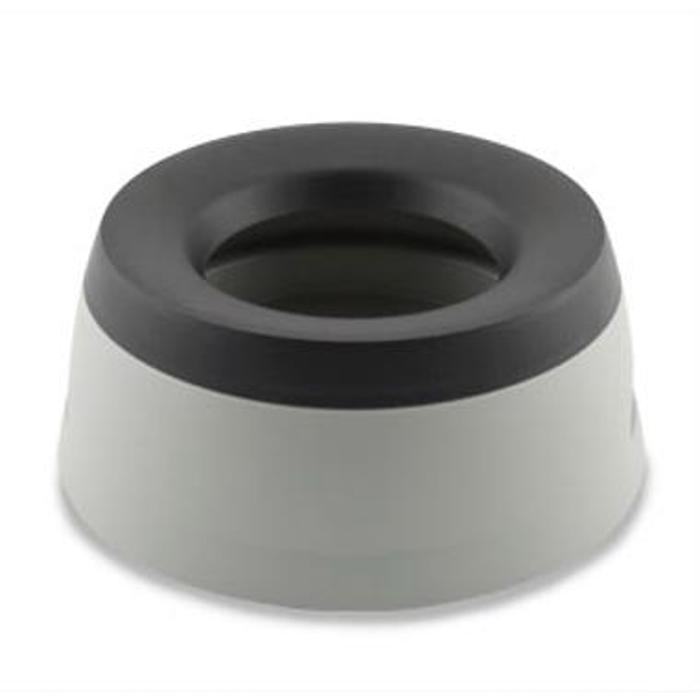
\includegraphics[width=2cm]{figs/obj_29_p2.jpg}} & \textbf{Low-complexity object}                \\
\toprule
                   & ``cup holder"                                   \\
                   & ``it is a bowl with a black portion on top"      \\
                   & ``football kicker's stand"                      \\
                   & ``portable toilet"                              \\
                   & ``it looks like an ash tray, but a bit shallow" \\
                   & ``looks like a dog bowl" \\
 \bottomrule
~ & ~ \\
  \toprule
\multirow{6}{*}{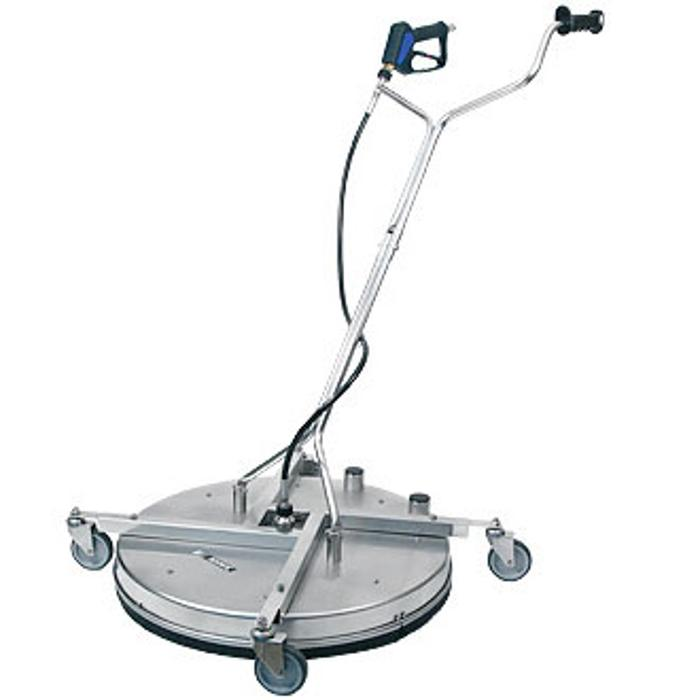
\includegraphics[width=1.8cm]{figs/obj_27_p2.jpg}} & \textbf{High-complexity object}               \\
\toprule
                   & ``a robotic carpet shampooer"                                   \\
                   & \multicolumn{1}{p{12cm}}{ ``it's a flat silver disk on rollers with what appear to be tall handlebars standing away from it at an angle"}                     \\
                   & ``a pressurized floor buffer on wheels"                                   \\
                   & ``it looks like a high tech metal detector on wheel."                                   \\
                   & ``it kinda looks like a portable lamp"                                \\  
                   & ``It is a machine with a circular stand and wheels, it has a metal handle"\\
   \bottomrule
\end{tabular}
\caption{Sample descriptions of a low- (top) and high- (bottom)  complexity objects.  Overall, descriptions were longer for high-complexity objects.}
\label{tab:sample_obj_descriptions}
\end{table}


Example descriptions for a low and high complexity object are presented in Table~\ref{tab:sample_obj_descriptions}. We considered two measures of length:  log number of characters and log number of words. Across objects, the mean length of description was  $M = 8.82$ words ($SD = 1.14$) and $M = 36.31$ characters ($SD = 4.69$).

 \begin{figure}
 \begin{center}
  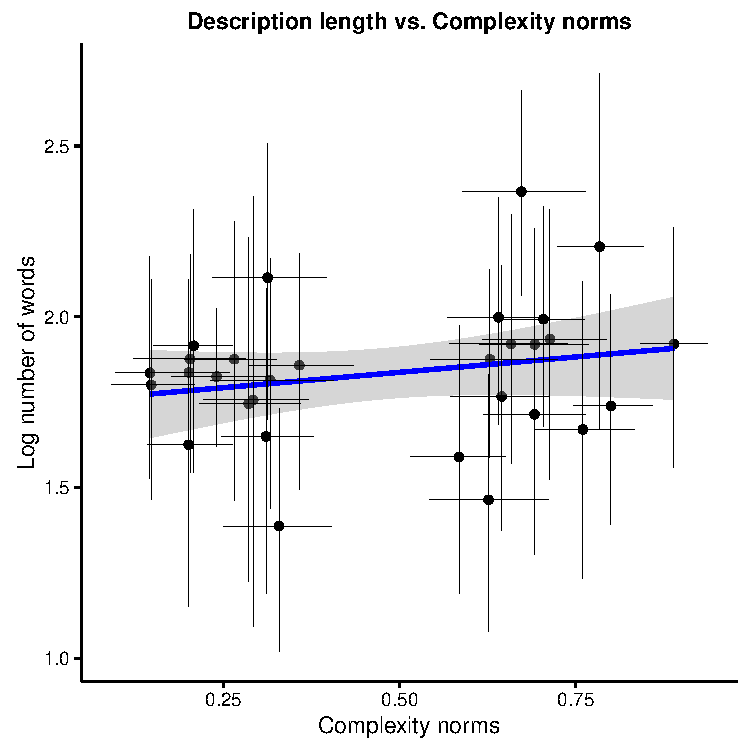
\includegraphics[width=4in]{figs/desc_length_word.pdf}
  \caption{\label{fig:desc_length} Relationship between description length and complexity norms. Error bars show  95\% confidence intervals.}
 \end{center}
\end{figure}


The key question was whether the description length was related to the psychological correlates of complexity measured in Chapter 2: Explicit ratings and study times.
To test this question we fit a  linear mixed-effect model predicting log number of words with complexity norms as a fixed effect, and a second model predicting log number of characters with study times as a fixed effect. As evident from Table~\ref{tab:sample_obj_descriptions}, participants varied considerably in the  syntactic construction of their descriptions as well as overall  length, making it important to control for this variability using a  mixed-effect model. The random effect structure included by-participant intercepts and by-trial slopes. There was a reliable relationship between log number of words and  complexity norms ($\beta=.2$, $t =2.8$; Fig~\ref{fig:desc_length}), and between number of words and study times ($\beta=.59$, $t =3.07$). The same pattern held for log number of characters. 

In the context of the Classical Theory of concepts, this result suggests a connection between conceptual complexity and number of primitives: More conceptually complex objects have longer descriptions, and thus more primitives. 

\section{Experiment 2a: Definitions of words}
Experiment 1 suggested objects that appear visually more complex are described with longer descriptions. The studies in Chapter 2, however, suggest that the construct of conceptual complexity extends beyond visual complexity to abstract word meanings. This predicts the length of a dictionary definition of a word should be correlated with the conceptual complexity of its meaning. In light of the complexity bias observed in Chapter 2, we also predict that words with more complex definitions should be longer and have definitions that are rated as more complex. In Experiment 2 we tested these predictions by presenting participants with the definition of low frequency English words  and asking them to rate the conceptual complexity of the definition.

We selected low frequency words for two reasons. First, because participants were unlikely to know the word associated with the definition, knowledge of a word's length was unlikely to affect the complexity judgement. Second, because the words were uniformly low frequency, this reduced the possibility that differences in word length were due to frequency, rather than conceptual complexity. 

\subsection{Methods}

\subsubsection{Participants} 
200 participants completed the task.

\subsubsection{Stimuli} 
We selected 100 dictionary definitions of low-frequency words (Table~\ref{tab:sample_word_defs}). 

\begin{table}[t!]
\centering

\begin{tabular}{ll}
\toprule
\textbf{Word} & \textbf{Definition}                \\
\toprule
   bissextile & ``a leap year"\\
   mussitation  &  \multicolumn{1}{p{12cm}}{ ``movement of the lips as if in speech but without accompanying sound"}    \\
   omphaloskepsis  &  \multicolumn{1}{p{12cm}}{ ``contemplation of one's navel as an aid to meditation"}                  \\
   parvis    &  \multicolumn{1}{p{12cm}}{ ``a court or enclosed space before a building"}                               \\
   sniddle      &  \multicolumn{1}{p{12cm}}{ ``long coarse grass"}     \\
   zarf     & \multicolumn{1}{p{12cm}}{ ``a holder, usually of ornamental metal, for a coffeecup without a handle"}                                 \\

 \bottomrule
\end{tabular}
\caption{Sample definitions of real English words used in Experiment 2.}
\label{tab:sample_word_defs}
\end{table}


\subsubsection{Procedure}
The task was identical to Experiment 9 in Chapter 2, except that participants were presented with definitions rather than words. Participants were first presented with instructions describing the norming task:
\begin{quote}
In this experiment, you will be shown the definition of a word and asked to decide how complex the meaning is. A word's meaning is simple if it is easy to understand and has few parts. An example of a simple meaning is ``brick.'' A word's meaning is complex if it is difficult to understand and has many parts. An example of a more complex meaning is ``engine.''
\end{quote}
For each definition, we then asked ``How complex is this definition?,'' and participants indicated their response on a 7-pt Likert scale anchored at ``simple'' and ``complex.'' The first two words were always ``ball'' and ``motherboard'' to anchor participants on the scale. Each participant rated a sample of 10 definitions. 

\subsection{Results and Discussion}
The central prediction is that definitions with more primitives in the definition, operationalized as the length of the definition, should be rated as conceptually more complex. To test this prediction, we fit a linear mixed-effect model predicting complexity ratings with log number of words in the definition as a fixed effect. The random effect structure included by-participant intercepts and by-trial slopes. As predicted, there was a strong relationship between complexity ratings and log number of words ($\beta=1.50$, $t =27.94$). The same pattern held for log number of characters.

A secondary prediction was that there should be a relationship between the length of the definition and the length of the word: If languages encode the conceptual complexity of a word's meaning in the length of the word, longer words should be associated with longer definitions. This prediction was not supported ($r=.05$, $p =.59$). Finally, we should also expect that  longer words should be associated with definitions rated as more complex. We fit the same mixed-effect model as above to test this prediction, except with log number of characters in the word as a fixed effect. There was a significant relationship between word length and rating judgements ($\beta=.52$, $t =2.86$), suggesting more complex definitions area associated with longer words. However, in a model with both word length and definition length as fixed effects, word length was no longer a reliable predictor of complexity ratings ($\beta=.18$, $t =1.19$).

In sum, we find a strong relationship between definition length and conceptual ratings, as predicted by Classical Theory of concepts: Longer definitions, with more primitives, are rated as more complex. We do not, however, find the predicted relationship between the conceptual complexity of the definition and word length, as would be predicted by the studies in Chapter 1.  One possible explanation for this null finding is that participants' complexity ratings were driven by the linguistic complexity of the definition, rather than its conceptual complexity. In other words, participants may have  rated longer definitions as more complex {\it because} they were longer, not because they were more conceptually complex. The current design does not allow us to distinguish these two possibilities. In Study 3, we try to address this confound more directly. 

\section{Experiment 2b: Definition mapping}.
If definition length is related to conceptual complexity and participants have a complexity bias, we predict that participants should be biased to map longer definitions on to  longer words. In Experiment 2b, we test this prediction in an experiment analogous to the word mapping experiments in Chapter 2. Participants were presented with a meaning---a definition---and asked to guess the translation of the meaning in an alien language from two possible alternatives, one long and one short. 

\subsection{Methods}
\subsubsection{Participants} 
200 participants completed the experiment.
\subsubsection{Stimuli} 
We used the normed definitions from Experiment 2a. The short novel words containing one syllable, and the long novel words contained three syllables. There were 10 short and 10 long novel words presented in random order. 

\subsubsection{Procedure}
Participants were first presented with the following instructions:
\begin{quote}
In this experiment, you will see the definition of a word. Your job is to guess what the translation of that word is in an alien language. You will make your guess by betting on two possible words in the alien language. Imagine you have a \$100 dollars. To place your bet, assign an amount to each of the words. Your bets must add to 100.
\end{quote}
Participants then viewed a definition and two possible alternative words, one short and one long. Participants selected a response by placing a numeric bet under each word.  Each participant rated 10 definitions in total. 

\subsection{Results and Discussion}
Correlated with conceptual ratings
correlated with definition length
IN model with both, mostly just defintion length.

Suggests participants just matching long definition to long word. Need better way to measure the primitives in. See Study 3.

\section{Study 3: McCrae feature norms}
The above approach is messy. 

\subsection{Methods}
\subsection{Results and Discussion}

\section{Study 4: Entropy of associates}
\subsection{Methods}

\subsection{Results and Discussion}

\section{Experiment 5a: Simultaneous frequency}
Both 
\subsection{Methods}
\subsubsection{Participants} 
477 participants completed the experiment.
\subsubsection{Stimuli} 
\subsubsection{Procedure}
We presented participants with 10 objects on a single screen. The objects were composed of a single geon. There were two types of objects. One object type appeared nine times and the second object type appeared once. After this training period, participants completed a forced choice mapping task, as in Studies 1 and 5. We presented a word that was either 2 or 4 syllables long and asked participants to make a judgment about whether the word referred to the low or high frequency object. Each participant completed a single mapping trial, and word length was manipulated between participants.

 \subsection{Results and Discussion}
 Selections between the two conditions did not differ (?2(1) = 0.02, p = .89).


\section{Experiment 5b: Sequential frequency}

\subsection{Methods}
\subsubsection{Participants} 
97 participants completed the experiment.
\subsubsection{Stimuli} 
\subsubsection{Procedure}
We manipulated object frequency by sequentially presenting objects. Participants saw 60 objects from the set of normed real objects one at a time. One object was presented 10 times and a second object was presented 40 times. Ten additional objects were included as fillers. After this training phase, participants completed a single mapping trial as in Experiment 5a. Word length was manipulated between participants.
\subsection{Results and Discussion}
Selections between the two conditions did not differ (?2(1) = 0.01, p = .92).

\section{Experiment 6: Facts}
\subsection{Methods}
\subsubsection{Participants} 
\subsubsection{Stimuli} 
\subsubsection{Procedure}
\subsection{Results and Discussion}

\section{Experiment 7: Concept variability}
\subsection{Methods}
\subsubsection{Participants} 
\subsubsection{Stimuli} 
\subsubsection{Procedure}
\subsection{Results and Discussion}







